% \documentclass[a4paper]{article}
\documentclass[a4paper,14pt]{extarticle}
\usepackage[utf8]{inputenc}


\usepackage{geometry}

\usepackage[mathcal]{euscript}

\usepackage{amsmath, amsfonts, amssymb, amsthm}
\usepackage{mathptmx}
\usepackage{algorithm2e}

\usepackage{graphicx, url}

\newcommand{\Fcal}{\mathcal{F}}
\newcommand{\Ncal}{\mathcal{N}}
\newcommand{\Rcal}{\mathcal{R}}
\newcommand{\Xcal}{\mathcal{X}}
\newcommand{\Ycal}{\mathcal{Y}}
\newcommand{\Real}{\mathbb{R}}
\newcommand{\cut}{\mathop{\mathtt{cut}}\nolimits}
\newcommand{\argmax}{\mathop{\mathtt{argmax}}\nolimits}
\newcommand{\argmin}{\mathop{\mathtt{argmin}}\nolimits}
\newcommand{\ex}{\mathop{\mathbb{E}}\nolimits}
\newcommand{\pr}{\mathop{\mathbb{P}}\nolimits}
\newcommand{\var}{\mathop{\text{var}}}
\newcommand{\one}{\mathbf{1}}

\usepackage[english, russian]{babel}
\newcommand{\eng}[1]{\foreignlanguage{english}{#1}}
\newcommand{\rus}[1]{\foreignlanguage{russian}{#1}}

\title{Preparation for the finals}
\author{Nazarov Ivan, \rus{101мНОД(ИССА)}\\the DataScience Collective}

\begin{document}
\maketitle

\selectlanguage{english}

\section{\rus{Общие вопросы программы}} % (fold)
\label{sec:general_questions}
\noindent\textbf{Q:}\rus{Классический и ранговый критерии для проверки гипотезы об
однородности двух выборок против альтернативы сдвига.}

\hfill\\\noindent\textbf{A:}
Consider two samples $X_1=(x_{1i})_{i=1}^{n_1}\sim F$ and $Y=(x_{2j})_{j=1}^{n_1}
\sim F(\cdot - \theta)$. We wan to check the following hypotheses $H_0: \theta=0$
versus an one of the following composite alternatives $H_1:\theta < 0$, $H_1:\theta > 0$,
or $H_1:\theta \neq 0$.

\paragraph{The classical Student criterion} % (fold)
\label{par:the_classical_student_criterion}

If $F = \Ncal(\cdot, \sigma^2)$, and samples $X_1$ and $X_2$ are independent, then
one can simply use the Gaussianity assumption to derive
$$ \hat{\theta} = \bar{X}_1 - \bar{X}_2
    \sim \Ncal(\theta, \sigma^2 (n_1^{-1} + n_2^{-1}))
    \,, $$
where $\bar{X}_k = n_k^{-1} \sum_{i=1}^{n_k} x_{ki}$. Since the variance is unknown,
one has to estimate it using the unbiased pooled sample estimate
$$ s^2
    = (n_1 + n_2 - 2)^{-1}\bigl(
        \sum_{i=1}^{n_1} (x_{1i} - \bar{X}_1)^2
        + \sum_{j=1}^{n_2} (x_{2j}- \bar{X}_2)^2
        \bigr)
    \,. $$
The since $\ex s^2 = \sigma^2$ and it is a quadratic form over Gaussian vectors,
we have $\sigma^{-2} s^2 \sim \chi^2_{n_1 + n_2 - 2}$. Moreover it could be shown
that it is independent of both $\bar{X}_1$ and $\bar{X}_2$. Hence, by definition
of the Student random variable we have
$$ T(X_1, X_2)
    = (\sigma^{-2} s^2)^{-\frac{1}{2}}
      (\sigma^2 (n_1^{-1} + n_2^{-1}))^{-\frac{1}{2}} \hat{\theta}
    = \frac{\hat{\theta}}{s \sqrt{n_1^{-1} + n_2^{-1}}}
    \sim t_{n_1 + n_2 - 2}
    \,. $$
Hence we have these tests for some significance level $\alpha$:\begin{itemize}
    \item Against $H_1:\theta < 0$: reject $H_0$ if $T(X, y) < t_{\alpha, n_1 + n_2 - 2}$;
    \item Against $H_1:\theta > 0$: reject $H_0$ if $T(X, y) > t_{1-\alpha, n_1 + n_2 - 2}$;
    \item Against $H_1:\theta \neq 0$: reject $H_0$ if $|T(X, y)| > t_{1-\frac{\alpha}{2}, n_1 + n_2 - 2}$;
\end{itemize}

% paragraph the_classical_student_criterion (end)
\paragraph{Wilcoxon criterion} % (fold)
\label{par:wilcoxon_criterion}
Consider the ranking function $R$, that for every sample $Z=(z_i)_{i=1}^l$, returns
the place of each observation in ordered $Z$, with ties resolved using average rank.

In the same setting as before, make a pooled sample $Z = X \| Y$, and compute its
ranks
$$ (\rho^z_k)_{k=1}^{n_1+n_2} = R((x_{1i})_{i=1}^{n_1}\|(x_{2j})_{j=1}^{n_2}) \,, $$
and take the sum of all ranks of the $Y$ sample in the pooled to get the Wilcoxon
statistic: $ W = \sum_{j=1}^{n_2} \rho^z_{n_1+j} $. Now, in the extreme case, if
all $Y$ is to the right of $X$ in the ordered pooled sample, then $W_{\text{min}}
= n_2 (n_2+1)\frac{1}{2}$. In another extreme case, when $Y$ is to the right of $X$,
we have $W_{\text{max}} = n_2(n_2 + 2n_1 + 1) \frac{1}{2}$.

In any case under the null hypothesis it is true that $ \ex W = \frac{n_2 (n_2 + n_1 + 1)}{2}$,
and the Wilcoxon statistic is symmetric around its mean: for all $c\in \mathbb{R}$
$$ \pr(W - \ex W \leq c) = \pr(W - \ex W \geq -c) \,, $$
and for sufficiently large $n_k$ we have the limiting Gaussianity:
$$ \frac{W - \ex W}{\sqrt{\sigma^2_W}} \sin \Ncal(0, 1) \,, $$
where 
$$ \sigma^2_W = \frac{n_1 n_2 (n_1+n_2+1)}{12} \,. $$
For samples with ties it is necessary to adjust the variance
$$ \sigma^2_W
    = \frac{n_1 n_2}{12} \biggl(n_1+n_2+1
        -\frac{\sum_{k=1}^l t_k(t_k^2-1)}{(n_1+n_2)(n_1+n_2+1)}
    \biggr) \,, $$
where $t_k$ is the numbers of tied values in the $k$-th group of the pooled sample.
Wilcoxon test is consistent for the considered composite alternatives, nonparametric,
and is robust (locally most powerful) in the class of rank-based tests of homogeneity
versus shift. When the Gaussianity assumptions hold (t-test is exact), it is asymptotically
efficient.

% paragraph wilcoxon_criterion (end)

\hfill\\\noindent\textbf{Q:}\rus{Классический и ранговый критерии для проверки гипотезы
об однородности двух выборок против альтернативы масштаба.}

\hfill\\\noindent\textbf{A:}
Consider two samples $X=(x_{1i})_{i=1}^{n_1}\sim F$ and $X_2=(x_{2j})_{j=1}^{n_2}
\sim F(\cdot\Delta^{-1})$. We wan to check the following hypotheses $H_0: \Delta=1$
versus one of the following composite alternatives $H_1: \Delta < 1$, $H_1: \Delta > 1$,
or $H_1: \Delta \neq 1$.

\paragraph{Classical Fisher Criterion} % (fold)
\label{par:classical_fisher_criterion}
Assume that $X_k \sim \Ncal(m_k, \sigma^2_k)$ iid and jointly independent. Under
the null we test $\sigma^2_1=\sigma^2_2$. The unbiased sample estimates of $\sigma^2$
are given by
$$ s^2_k = (n_k-1)^{-1} \sum_{i=1}^{n_k} (x_{ki} - \bar{X}_k)^2 \,,$$
whence the test statistic ratio
$$ T(X_1, X_2)
    = \frac{\sigma^{-2}_1 s^2_1}{\sigma^{-2}_2 s^2_2}
    = \frac{s^2_1}{s^2_2}
    \sim F(n_1-1, n_2-1) \,, $$
has the Fisher distribution, since it is a ratio of independent $\chi^2$.

The critical and confidence regions for $T(X_1, X_2)$ depend on the alternative
hypothesis, and are as follows: \begin{itemize}
    \item $H_1: \sigma^2_1 < \sigma^2_2$, then fail to reject $H_0$ if
    $$ [(F_{1-\alpha}(n_2-1, n_1-1))^{-1}, +\infty) \,;$$
    \item $H_1: \sigma^2_1 > \sigma^2_2$, then fail to reject $H_0$ if
    $$ [0, F_{1-\alpha}(n_1-1, n_2-1)] \,; $$
    \item $H_1: \sigma^2_1 \neq \sigma^2_2$, then fail to reject $H_0$ if
    $$ [(F_{1-\alpha}(n_2-1, n_1-1))^{-1}, F_{1-\alpha}(n_1-1, n_2-1)] \,; $$
\end{itemize}

% paragraph classical_fisher_criterion (end)

\paragraph{Ansari-Bradley test} % (fold)
\label{par:ansari_bradley_test}
Suppose the samples $X_1\sim F$ and $X_2\sim F(\cdot\Delta^{-1})$ are idd, jointly
independent, that distribution $F$ is continuous. Suppose without the loss of generality
that the sample medians coincide (just subtract them).

Take the order statistics of the pooled sample $X = X_1 \| X_2$, the carry out two
sided ranking: assign rank $1$ to the smallest and the largest, rank $2$ to $X_{(2)}$
and $X_{(N-1)}$, and so on. Here $N=n_1+n_2$. The Ansari-Bradley statistic $A$ is
defined as the sum of the two-sided ranks of the sample $X_2$ in the pooled sample
$X$. Similarly to the Wilcoxon test, the distribution of this statistic under the
null is symmetric around the mean, and asymptotic normality holds the for the standardized
statistic:
$$ \frac{A - \ex A}{\sqrt{\var A}} \sim \Ncal(0, 1) \,, $$
where the mean is
$$ \begin{cases}
    \frac{n_1(N+2)}{4}, &\text{ if } N \text{is even}\\
    \frac{n_1(N+1)^2}{4 N}, &\text{ otherwise}\\
\end{cases} \,, $$
and the variance is given by
$$ \begin{cases}
    \frac{n_1 n_2(N+2)(N-2)}{48(N-1)}, &\text{ if } N \text{is even}\\
    \frac{n_1(N+1)(N^2+3)}{48 N^2}, &\text{ otherwise}\\
\end{cases} \,. $$

The test critical regions: \begin{itemize}
    \item one-tail alternative $H_1:\gamma < 1$: reject $H_0$ is $A\geq A_\alpha$;
    \item one-tail alternative $H_1:\gamma > 1$: reject $H_0$ is $A\leq A_{1-\alpha} - 1$;
    \item two-tail alternative $H_1:\gamma \neq 1$: reject $H_0$ unless
    $A_{1-\frac{\alpha}{2}} - 1 \leq A \leq A_\frac{\alpha}{2}$;
\end{itemize}
where $\gamma$ is the ratio of scales of $X_2$ and $X_1$.
The intuition is that if the typical scale of the sample $X_2$ is larger than that
of $X_1$, then the two-sided ranks of $X_2$ would be on average much lower than
those of $X_1$.

% paragraph ansari_bradley_test (end)

\hfill\\\noindent\textbf{Q:}\rus{Постановка задачи однофакторного дисперсионного
анализа. Оценивание контрастов в модели однофакторного дисперсионного анализа.}

\hfill\\\noindent\textbf{A:}

\hfill\\\noindent\textbf{Q:}\rus{Применение непараметрических методов в задаче однофакторного
дисперсионного анализа.}

\hfill\\\noindent\textbf{A:}

\hfill\\\noindent\textbf{Q:}\rus{Кластеризация. Основные методы кластеризации.
Типы исходных данных. Визуализация кластеров.}

\hfill\\\noindent\textbf{A:}

\hfill\\\noindent\textbf{Q:}\rus{Кластеризация методом K-средних. Основные алгоритмы.
Инициализация. Аномальные кластеры.}

\hfill\\\noindent\textbf{A:}

\hfill\\\noindent\textbf{Q:}\rus{Иерархическая кластеризация. Агломеративные и
дивизионные методы.}

\hfill\\\noindent\textbf{A:}

% section general_questions (end)


\section{\rus{Упорядоченные множества в анализе данных}} % (fold)
\label{sec:ordered_sets}

\noindent\textbf{Q:}\rus{Свойства бинарных отношений. Отношения частичного
порядка, эквивалентности, толерантности. Отношения строгого порядка и
покрытия, связанные с отношением частичного порядка. Графы отношений,
диаграммы частичного порядка. Полурешетки, решетки. Два определения решеток
и теорема об их эквивалентности.}

\hfill\\\noindent\textbf{A:}
A binary relation on $\Omega$ is a subset $R\subseteq \Omega\times \Omega$.
The following properties:
\begin{description}
    \item[Reflexivity:] $(x, x)\in R$ for all $x\in\Omega$;
    \item[Anti-reflexivity:] $(x, x)\notin R$ for all $x\in\Omega$;
    \item[Symmetry:] $(x, y)\in R$ implies $(y, x)\in R$;
    \item[Asymmetry:] $(x, y)\in R$ implies $(y, x)\notin R$;
    \item[Anti-symmetry:] $(x, y), (y,x)\in R$ implies $y=x$;
    \item[Transitivity:] $(x,y), (y,z)\in R$ imply $(x,z)\in R$;
    \item[Totality (Completeness):] $\forall x, y\in \Omega$ either $(x,y)\in R$,
    or $(y,x)\in R$, or both.
\end{description}
Binary Relations are equivalent to graphs: if $R$ is a binary relation on $\Omega$
then its graph is $G = (V, E)$ for $V$ -- the set of all elements of $\Omega$
participating in $R$.

\noindent Relation composition: for two binary relations $R_1$ and $R_2$ on $\Omega$
$$ R_1\circ R_2
    = \{(x,z)\in \Omega\times\Omega
        \,:\, \exists y\in \Omega\, (x,y)\in R_1, (y,z)\in R_2\}
    \,. $$
\noindent Transitive closure:
$R^T = \bigcap_{L\in [R]} L$, for $[R]$ -- the set of all transitive binary
relations on $\Omega$ that cover $R$. In fact $R^T = \bigcup_{n\geq1} R^n$,
where $R^n = R\circ \ldots \circ R$ -- $n$ times. Indeed, suppose $R\subseteq M$
for some transitive rlation $M$, then for $(a,b)\in R^T$ there is $n\geq 1$
such that $(a,b)\in R^n$, whence $\exists (u_i)_{i=0}^n\in R$ with $(u_{i-1}, u_i)\in R$
such that $u_0=a$ and $u_n=b$. Since $R\subseteq M$, $(a,b)\in M$ by transitivity.

\noindent Examples: \begin{description}
    \item[Equivalence:] a reflexive, symmetric and transitive relation.
    \item[Tolerance:] a reflexive, symmetric relation.
    ``Equal within threshold'': $\{(a,b)\in \mathbb{R}\,:\, |a-b|\leq \epsilon\}$
    (``likeness'', ``similarity'').
    \item[Quasi-order (preorder):] reflexive and transitive relation.
    ``being isomorphic to a subgraph'': graph isomorphism, $G_1 \sim G_2$, is when
    there is a bijection $\phi:V_1\mapsto V_2$ with $(\phi(u),\phi(v))\in E_2$ iff
    $(u,v)\in E_1)$.
    \item[Partial order:] a reflexive, anti-symmetric, transitive relation.
    $(\mathbb{N}, \leq)$ on natural numbers is total, $(\mathcal{P}(\Omega),
    \subseteq)$ -- partial.
    \item[Strict order:] $(P, \leq)$ -- poset. A strict order is $(P, <)$ such
    that $a<b$ iff $a\leq b$ and $a\neq b$. Strict orders are anti-reflexive,
    asymmetric and transitive.
    \item[Covering relation:] $(P, \leq)$ -- poset. A covering relation is $(P, \prec)$
    such that $a\prec b$ iff $a\leq b$, $a\neq b$ and there is no $z\in P$ with $z\neq a,b$
    and such that $a\leq z\leq b$. Gives rise to Hasse diagrams (fig.~\ref{fig:hasse})
    of partial orders, which are used extensively in FCA.
\end{description}
\begin{figure}
    \centering
    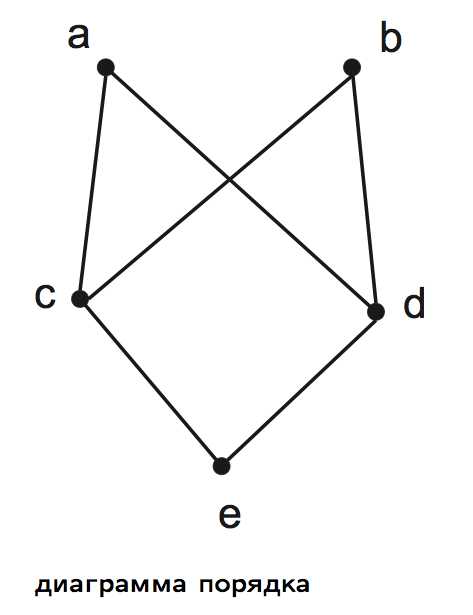
\includegraphics[width=0.35\textwidth]{hasse.png}
    \label{fig:hasse}
    \caption{a hasse diagram.}
\end{figure}

Algebraically a semi-lattice is pair $(L, \diamond)$ such that $\diamond: L\times L \to L$
is idempotent ($a\diamond a=a$), commutative ($a \diamond b = b \diamond a$) and associative
($a \diamond (b \diamond c) = (a \diamond b) \diamond c$). Natural partial order $a\leq b$
iff $a\diamond b = a$ (join).

From the order-theoretic approach, a join semi-lattice is a poset $(L, \leq)$ such
that the supremum (the least upper bound) $\sup\{x, y\}$ exists and unique for every
pair of $x, y \in L$. Similarly, a meet semi-lattice is a poset with a well-defined
pairwise infimum operation (uniqueness). These definitions are equivalent. (see.
\textbf{p.~5} of the notes).

A lattice $(L, \wedge, \vee)$ imposes an extra restriction on the operators:
$$ x = x \wedge (x\vee y) = x \vee ( x\wedge y) \,, $$
called ``absorption''. Note that $(L, \wedge)$ is a join semi-lattice and $(L, \vee)$
is a meet semi-lattice. The natural order on $(L, \wedge, \vee)$ is defined as
$a\leq b$ iff $a\wedge b=a$ (or $a\vee b = b$). A lattice $(L, \wedge, \vee)$ is
modular iff
$$ x\leq z \Rightarrow x \vee (y\wedge z) = (x \vee y ) \wedge z\, \forall y\,. $$

A lattice is distributive iff its Hasse diagram has neither diamonds, nor pentagons.
A lattice is modular iff its Hasse diagram contains no pentagons (fig.~\ref{fig:lattice_pen_di}).
\begin{figure}
    \centering
    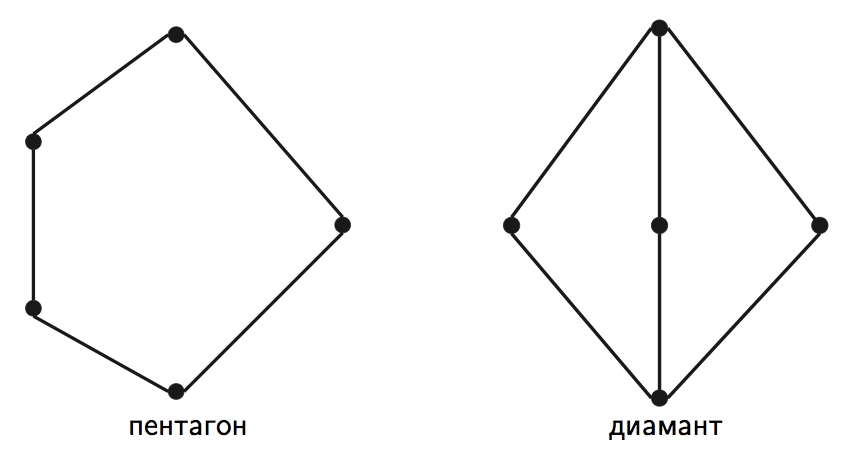
\includegraphics[width=0.35\textwidth]{pents_and_diamonds.png}
    \label{fig:lattice_pen_di}
    \caption{Pentagrams and diamonds.}
\end{figure}

\hfill\\\noindent\textbf{Q:}\rus{Соответствие Галуа, задаваемое бинарным отношением. Оператор
замыкания. Решетки формальных понятий, основная теорема анализа формальных понятий
(АФП): представимость полных решеток решетками понятий. Диаграмма решетки понятий
(граф отношения покрытия).}

\hfill\\\noindent\textbf{A:}
For the Galois connection see \textbf{p.~8}, for closure operator note that it is
defined as the composition of maps of the Galois connection see.~8-9. In general
a closure  operator (not the topological closure) has the following properties:
$[\cdot]: (P, \leq) \mapsto (P, \leq))$ is a closure operator if it is idempotent
($[[a]]=[a]$), extensive ($a\leq [a]$), and monotonic ($[a]\leq [b]$ whenever
$a\leq b$).

\noindent For concept lattices see \textbf{p.~10} and the complete lattice equivalence
see \textbf{p.~11-13}.

\hfill\\\textbf{Q:}\rus{Признаковые импликации в контексте. Базис импликаций Дюкена-
Гига (на основе псевдосодержаний) и генераторный базис. Импликации в контексте и
функциональные зависимости в теории реляционных баз данных (двусторонняя сводимость).}

\hfill\\\textbf{A:}
To summarize, in implication on a context $(G, M, I)$ is a pair $A, B\subseteq M$,
denoted by $A\to B$, if $A'\subseteq B'$ (or $B\subseteq  A$), i.e. all objects that
have all attributes from $A$ also have every attribute from $B$: for all $g\in G$
$$ A\subseteq g' \Rightarrow B \subseteq g'\,, $$
for such $A, B$. For details on implications, and Armstrong rules refer to \textbf{p.~15-19}
of the notes. Implication bases are covered in \textbf{p.~19-21} of the notes.

Based on lecture slides (lecture 5 slides 3-5). A multivalued context is $4$-tuple
$(G, M, W, I)$ with $W$ being the feature value set, $I\subseteq G\times M \times W$
is such that $(g,m,w), (g,m,v)\in I$ implies $w=v$ ($I$ is a map $G\times M\mapsto W$).
An attribute $m$ is complete if for any $g \in G$ there exists $w\in W$ with $(g,m,w)
\in I$. A multivalued context id complete if all its features are complete.
Each feature $m\in M$ in such context can be identified with a map $\phi_m:G\mapsto W$
(shorthand $m(\cdot) = \phi_m(\cdot)$) with $(g, m, m(g))\in I$ for all $m\in M$
and $g\in G$.

A functional dependence $X\mapsto Y$, $X, Y\subseteq M$ in a complete multivalued
context $(G, M, W, I)$ takes place if for each pair $g, h\in G$
$$ (m(g) = m(h)\,,\, \forall m\in X)
    \Rightarrow (n(g) = n(h)\,,\, \forall n\in Y)
    \,. $$
See \textbf{p.~24} of the notes.

Each complete multivalued context $K = (G, M, W, I)$ it is possible to define a context
$K_N = (\mathcal{P}_2(G), M, I_N)$, where $\mathcal{P}_2(G)$ is the set of all unordered
pairs of distinct elements of $G$ and $I_N$ is given by
$$ (\{g, h\}, m) \in I_N
    \Leftrightarrow m(g) = m(h)
    \,. $$
The a multivalued context $K$ has a functional dependence $X\mapsto Y$ iff the induced
context $K_N$ has an implication $X\to Y$.

For a context $K=(G, M, I)$ it is possible to construct a multivalued context
$K_W$ such that the implication $X\to Y$ takes place in $K$ iff $K_W$ has a functional
dependence $X\mapsto Y$. For example, fig.~\ref{fig:multivalued}:
\begin{figure}
    \centering
    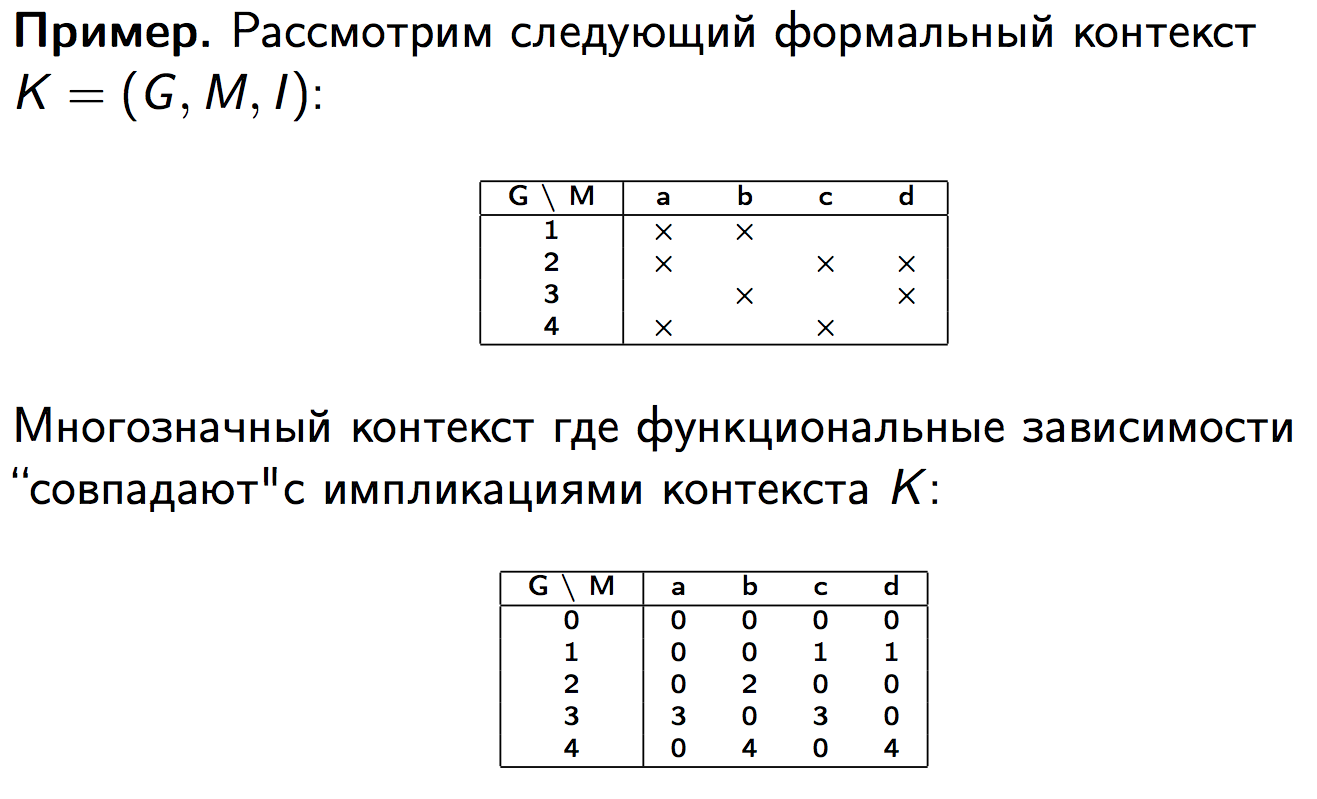
\includegraphics[width=0.5\textwidth]{multivalued.png}
    \label{fig:multivalued}
    \caption{A context and a multivalued context.}
\end{figure}
For further details on the multivalued contexts see \textbf{p.~24-25} of the notes.

\hfill\\\textbf{Q:}\rus{Ассоциативные правила как метод майнинга данных. Поддержка
и достоверность ассоциативных правил. Базис ассоциативных правил и его связь с диаграммой
решетки понятий.}

\hfill\\\textbf{A:}
For implications, support and confidence refer to \textbf{p.~21-22} of the notes.
An example application is purchase recommendations, near-duplicate documents clustering,
et c.

The ``lift'' of an association rule $A\to B$ is defined as 
$$ \mathtt{lift}(A\to B)
    = \frac{\mathtt{supp}(A\cup B)}{\mathtt{supp}(A)\cdot \mathtt{supp}(B)}
    \,, $$
and measures the departure from independence, The close the ``lift'' is to $1$,
the more likely that there is no underlying connection between $A$ and $B$. Interesting
cases are when the lift is greater than $1$. 

Association rules mining is performed in two steps: \begin{enumerate}
    \item Frequent itemset mining: detectin all $F \subseteq M$ with sufficient
    support $\mathtt{supp}(F)\geq \alpha$;
    \item Construction of association rules based on them.
\end{enumerate}

\noindent ``Apriori'' [Agrawal, Srikantl 1994] algorithm (alg.~\ref{alg:apriori})
finds all association rules in a context $(G, M, I)$ that have at least the specified
level of support ($\frac{|(A\cup B)'|}{|G|}$), and confidence ($\frac{|(A\cup B)'|}{|A'|}$).
The main insight of the algorithm is that if itemsets (of $M$) are related $A\subseteq B$
then $B'\subseteq A'$ -- the subsets are more frequent, while the supersets are less
frequent. This limits the exponentially large search space, and yields a nice, yet
computationally intensive algorithm.
\begin{algorithm}
    \caption{Aprirori algorithm for frequent itemset mining.}\label{alg:apriori}
    \SetKwInOut{Input}{input}\SetKwInOut{Output}{output}
    \Input{A formal context $K=(G, M, I)$, $(M, \leq)$ -- poset, minimal support $\alpha$.}
    \Output{All frequent itemsets.}
    \BlankLine
    $C_1 \leftarrow \{\{m\}\,:\, m\in M\}$\;
    \While{$C_n\neq\emptyset$}{
        \tcc{$F_n$ -- frequent itemsets of size $n$}
        $F_n \leftarrow \{f \in C_n \,:\, \mathtt{supp}(f) \geq \alpha\}$\;
        % $C_{n+1} \leftarrow \mathtt{AprioriGen}(F_n)$\;
        \tcc{Generate all candidate supersets in canonical order.}
        $C_{n+1} \leftarrow \{ p\|q_n\,:\,
            \forall\,p,q\in F_n \text{ with } (p_i)_{i<n} = (q_i)_{i<n}, p_n \leq q_n \}$\;
        \tcc{Eliminate candidate itemsets with infrequent subsets.}
        \ForEach{$c\in C_{n+1}$}{
            \ForEach{$s\in \mathcal{P}(c), |s| = n$}{
                \If{$s\notin F_n$}{
                    $C_{n+1} \leftarrow C_{n+1} \setminus \{c\}$\;
                    break\;
                }
            }
        }
        $i\leftarrow i+1$\;
    }
    Return $\bigcup_{n\geq1} F_n$\;
\end{algorithm}

A formal concept in association rules mining, is such a frequent itemset $F\subseteq M$
that $\mathtt{supp}(F)\geq \alpha$, but for all $F\subseteq P$ we have $\mathtt{supp}(P)
< \alpha$ (a kind of a maximal subset). Alternative algorithm from [Flach] is presented
in alg.~\ref{alg:maximal_flach}. It generates the maximally frequent itemset frontier
(anti-chain) in the full concept lattice of the context $K$ (fig.~\ref{fig:assoc_rules_lattice}).

\begin{algorithm}
    \caption{Maximal frequent itemset mining.}\label{alg:maximal_flach}
    \SetKwInOut{Input}{input}\SetKwInOut{Output}{output}
    \Input{A formal context $K=(G, M, I)$, minimal support $\alpha$.}
    \Output{All maximal frequent itemsets.}
    \BlankLine
    $M \leftarrow \emptyset$\;
    Initialize a priority queue $Q$ by $Q\leftarrow \{\emptyset\}$\;
    \While{$Q$ is not empty}{
        $I\leftarrow \mathop{\mathtt{top}} Q$\;
        $\text{max} \leftarrow \top$\;
        \ForEach{$P$ with $I\subseteq P$ and $|P| = |I|+1$}{
            \If{$\mathtt{supp}(P)\geq \alpha$}{
                $\text{max} \leftarrow \bot$\;
                \If{$P\notin Q$}{
                    Add $P$ to the bottom of $Q$ and prioritize by $P$'s support\;
                }
            }
        }
        \If{$\text{max}=\top$}{
            $M\leftarrow M \cup \{I\}$\;
        }
    }
    Return $M$\;
\end{algorithm}

\begin{figure}
    \centering
    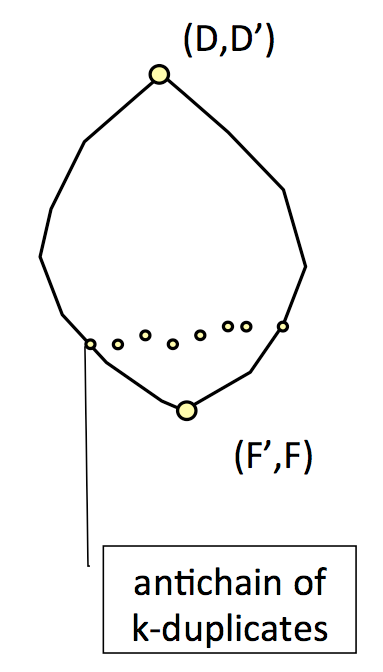
\includegraphics[width=0.25\textwidth]{assoc_rules_sublattice.png}
    \label{fig:assoc_rules_lattice}
    \caption{When grown with respect to $M$, the frequent itemset frontier
    exands from $(F', F)$.}
\end{figure}

Extraction of association rules from the set of frequent itemsets $\Fcal$ is done by
pruning the rules $P\to F\setminus P$, for $P\subseteq F$ with the minimal confidence
requirement:
$$ \mathtt{conf}(P \to F\setminus P)
    = \frac{\mathtt{supp}(F)}{\mathtt{supp}(P)} \geq \beta
    \,. $$
Note that one-element sets have the highest support, and thus rules of the form 
$f\to F\setminus \{f\}$ for any $f\in F$ have the lowest confidence. Furthermore,
all supersets of a high-support $P$ have, lower support, and thus higher confidence.
This idea yields a depth-first procedure for association rules construction.

\hfill\\\textbf{Q:}\rus{ДСМ-метод в терминах решеток понятий: гипотезы и классификация.
Соотношение ДСМ-гипотез и импликаций. Алгоритмы построения множества всех понятий (полный
перебор и ``Замыкай по одному'').}

\hfill\\\textbf{A:}
\noindent For the JSM method see the \textbf{p.~22-23} of the notes.

\noindent Consider a formal context $K=(G, M, I)$ with a complete order
$(G, \leq)$. Recall that a formal concept is a pair $(A, B)$ such that $A'=B$ and
$B'=A$. Then such pairs are naturally partially ordered by set inclusion (due to
anti-monotonicity of the Galois operators). Put $(A, B) \preceq (P, Q)$ iff $A\subset P$.
The key insight of CbO is that it in order to avoid exhaustive search, the virtual
concept lattice should be traversed in depth-first manner and in special order. In
particular the formal concepts are generated in lexicographic order (a canonical
generation), so that when a closure yields an out-of-order concept, the sub-lattice
of this concept is no longer traversed, because this exact concept has already been
generated by some other closure. The extent-based CbO algorithm is presented in
alg.~\ref{alg:cbo}, where $g^\leq = \{h\in G\,:\,h\leq g\}$ for any $g\in (G, \leq)$.
The full set of formal concepts is given by
$$ \mathtt{concepts}
    \leftarrow \mathtt{CbO}\bigl((\emptyset'', \emptyset'); K\bigr)
    \,. $$
For an intent based CbO, just reverse the roles (polarity) of $G$ and $M$ in the
description and the algorithm. This is due to the duality of the concept lattices.
\begin{algorithm}
    \caption{Intent based Close by One algorithm for $K$.}\label{alg:cbo}
    \SetKwInOut{Input}{input}\SetKwInOut{Output}{output}
    % A poset $(P, \leq)$, and a closure operator $[\cdot]: (P, \leq)\mapsto (P, \leq)$.
    \Input{A formal context $K$, a formal concept $(A, B)$.}
    \Output{A list of immediate descendant formal concepts $(P, Q)$ with $(A, B) \prec
    (P, Q)$.}
    \BlankLine
    $\mathtt{concepts} \leftarrow \{(A, B)\}$\;
    \For{$g \in G \setminus A$}{
        $(P, Q) \leftarrow \bigl((A \cup \{g\})'', (A \cup \{g\})'\bigr)$\;
        \tcc{Note that $B \cap \{g\}' = (A\cup \{g\})'$}
        \If{$\min\{P\setminus A\} \geq g$}{
        \tcc{or, equivalently, $(P\setminus A) \cap g^\leq$ is empty}
            $\mathtt{successors} \leftarrow \mathtt{CbO}((P, Q); K)$\;
            \tcc{these are the immediate successors to $(A, B)$}
            $\mathtt{concepts} \leftarrow \mathtt{concepts}
                                          \cup \mathtt{successors}$\;
        }
    }
    Return $\mathtt{concepts}$\;
\end{algorithm}
The recursion depth is no larger than $|G|$, and it is possible to make it into an
iterative algorithm by explicitly stroing the recursion tree, fig.~\ref{fig:cbo_tree}.
The complexity of this algorithm is output-dependent and given by:
\begin{description}
    \item[time complexity:] $\mathcal{O}(|\mathcal{B}(K)|\cdot |G|^2 \cdot |M|)$;
    \item[delay:] $\mathcal{O}(|G|^3 \cdot |M|)$;
    \item[space complexity:] $\mathcal{O}(|\mathcal{B}(K)|\cdot(|M| + |G|^2)
                                          + |G| \cdot |M|)$;
\end{description}
where $\mathcal{B}(K)$ is the formal concept lattice of $K$. Indeed, the closure
operation and finding the minimal element requires $\mathcal{O}(|G| \cdot |M|)$,
the loop is repeated at most $|G|$ times and the number of recursive calls is exactly
$|\mathcal{B}(K)|$. The delay is such, because before while going all the way down
over the lattice, the algorithm passes through at most $|G|$ layers within which
it has to make at most $|G|$ closures. The algorithm requires $|G| \cdot |M|$ space
for the context, and $|\mathcal{B}(K)|\cdot(|M| + |G|^2)$ for the lattice (with
connections and concepts).
(c.f. Kuznetsov, Sergei O., and Sergei A. Obiedkov. ``Comparing performance of algorithms
for generating concept lattices.'' Journal of Experimental \& Theoretical Artificial
Intelligence 14.2-3 (2002): 189-216.)
\begin{figure}
    \centering
    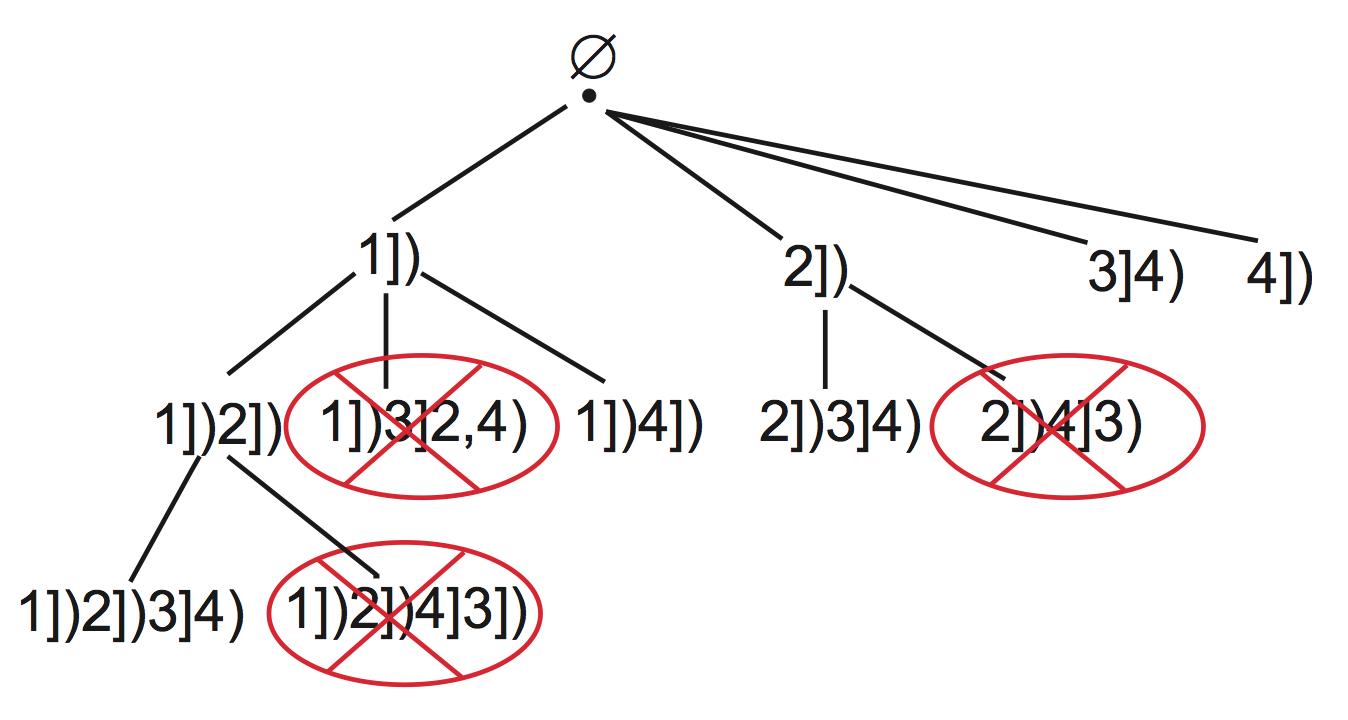
\includegraphics[width=0.5\textwidth]{cbo_tree.png}
    \label{fig:cbo_tree}
    \caption{Extent-based CbO recursion tree.}
\end{figure}

% section ordered_sets (end)

\section{\rus{Методы машинного обучения и майнинга данных}} % (fold)
\label{sec:mldm}

\noindent\textbf{Q:}\rus{Задача классификации.  Методы 1-Rule и ближайшего соседа
(kNN). Методы оценки качества. Скользящий контроль (crossvalidation). Точность и
полнота. ROC-кривые.}

\hfill\\\textbf{A:}
The problem of supervised learning is stated as follows. Suppose we are given a
domain of objects $\Xcal$, a range of labels $\Ycal$, and a finite sample $(x, y_x)_{x\in S}$
for some unknown (or even random) association $y:\Xcal\mapsto\Ycal$. The goal is
to learn an hypothesis (algorithm) $a:\Xcal\mapsto\Ycal$, that is able to generalize
the given sample of the association to never before seen objects $\Xcal$ (extrapolate
$y(\cdot)$). Classification is a supervised learning problem with a finite range
$\Ycal$ (as opposed to regression).

The standard classification loss function $L:\Ycal\times \Ycal \to\Real$ is the
$0-1$ loss, given by $L(p, y) = 1_{p\neq y}$. The empirical risk is the sample
average loss
$$ \hat{\Rcal}_S(h(\cdot))
    = |S|^{-1} \sum_{x\in S} L(h(x), y_x)
    = \ex_S L(h(x), y_x)
    \,, $$
where $\ex_S$ denotes the expectation over the empirical measure induced by $S$.

Theoretically, it would be great to learn such a classifier $h:\Xcal\mapsto\Ycal$,
that minimizes the theoretical risk $\Rcal(h(\cdot)) = \ex_D L(h(x), y_x)$, where
$D$ is the true unknown distribution of the data on $\Xcal\times \Ycal$. However,
this functional is unavailable, and thus we have to get by minimizing the empirical
risk, which is known to be an approximation of the theoretical risk due to the Law
of Large Numbers. We do this, hoping that the $\hat{h}_S = \argmin_h \hat{\Rcal}_S(h(\cdot))$
also more-or-less minimizes the theoretical risk.

Full available sample is usually split in three subsamples, making sure that the
class balance is preserved: \begin{itemize}
    \item train sample -- to train the model, and carry out limited tuning;
    \item validation sample -- to tune hyper-parameters of the learning algorithm;
    \item test sample -- to assess the generalization error;
\end{itemize}

\paragraph{$1$-rule classification} % (fold)
\label{par:1R_classification}
The general idea is to use extremely simple hypothesis class, which consists of
decision stumps. $1$-rules are learnt from the train sample by using the following
algorithm [Witten et al.; Data Mining, 2011] (alg.~\ref{alg:1R_algorithm}):
\begin{algorithm}
    \caption{One-Rule learning}\label{alg:1R_algorithm}
    \SetKwInOut{Input}{input}\SetKwInOut{Output}{output}
    \Input{Training sample $(x, y_x)_{x\in S}$, with each $x\in S$ possessing
    of the common feature set $\Fcal$ and having the value $f(x)$ for all $f\in\Fcal$.}
    \Output{The $1$-Rules with the smallest empirical error rate.}
    \BlankLine
    $R \leftarrow \emptyset$\;
    \ForEach{feature $f\in \Fcal$}{
        \ForEach{value $v\in \{f(x)\,:\, x\in S\}$}{
            $c_{fv} \leftarrow \argmax_{y\in \Ycal}
                    |\{ x\in S\,:\, f(x) = v\,, y_x = y \}|$\;
            $R \leftarrow R \cup \{ (f, v) \to c_{fv} \}$\;
        }
    }
    Choose the rules with the smallest error rate\;
\end{algorithm}

% paragraph 1R_classification (end)

\paragraph{$k$-NN classification} % (fold)
\label{par:kNN_clssification}

$k$-nearest neighbours classification is an similarity based classification method,
which in essence assigns to a new observation the dominant class label in its $k$-
neighbourhood with respect to some dissimilarity measure (distance, cosine, et c.)

Formally, let $\Xcal$ be endowed with a dissimilarity measure $d:\Xcal\times \Xcal
\mapsto \Real$. The training dataset is a sample from some $y:\Xcal\mapsto \Ycal$,
and is given by $(x, y_x)_{x\in S}$. Let $N_\epsilon^d(v)$ for some $v\in \Xcal$
be the set of all points in $S$ with distance to $v$ less than $\epsilon$ according
to $d$:
$$ N_\epsilon^d(v) = \{x\in S\,:\, d(v, x) \leq \epsilon \} \,, $$
and let $N_k^d(v)$ be the $k$-neighbourhood of $v$ ($k$ closest neighbours of $v$
in $S$). Then the predicted class label of $v$ is given by
$$ \hat{h}(v) = \argmax_{p\in \Ycal} \sum_{x\in N_k^d(v)} 1_{y_x = p}\,. $$
Straightforward modification of the $k$-NN decision rule is the introduction of
distance-based weights $w_{(i)} = 1 + \frac{1-i}{k}$ for the $i$-th nearest neighbour.

The nearest neighbour classification algorithm is the $k$-NN for $k=1$, and basically
propagates to a new object $v\in \Xcal$ the label of the training example most similar
to it.

% paragraph kNN_clssification (end)

\hfill\\\textbf{Q:}\rus{Задача классификации.  Метод Naïve Bayes. Методы оценки
качества. Скользящий контроль (crossvalidation). Точность и полнота. ROC-кривые.}

\hfill\\\textbf{A:}
Consider a training dataset $(x, y_x)_{x\in S}$ with label assignment $y:\Xcal\mapsto
\Ycal$, and each object having features $f\in \Fcal$ (being feature mappings from
$\Xcal$ to some label space, $\Real$, for example). The central assumption of the
Na\"ive Bayes classifier is independence of the feature mappings: elements of the
vector $(f(x))_{f\in \Fcal}$ are independent for any $x\in S$.

In order to classify a new object $v\in \Xcal$ (for which the feature mappings are
well defined) NB classifier does the following (Maximum a posteriori decision rule):
$$ \hat{y}_v
    = \argmax_y \pr_S\bigl(y_x = y \,|\,
            (f(x))_{f\in \Fcal} = (f(v))_{f\in \Fcal}\bigr)
    \,, $$
where $\pr_S$ is the posterior probability given by
$$ \pr\bigl(y_x = y \,|\, \forall f\in \Fcal\, f(x) = f(v)\bigr)
    = \frac{\pr\bigl(\forall f\in \Fcal\, f(x) = f(v) \,|\, y_x = y\bigr)
            \pr(y_x = y)}
        {\pr\bigl((f(x))_{f\in \Fcal} = (f(v))_{f\in \Fcal}\bigr)}
    \,. $$
The main assumption of NB is that conditional on the class label the feature distribution
factorizes into
$$ \pr\bigl((f(x))_{f\in \Fcal} = (f(v))_{f\in \Fcal} \,|\, y_x = y\bigr)
    = \prod_{f\in \Fcal} \pr_f(f(x) = f(v) \,|\, y_x = y)
    \,. $$ 

The class prior can be assumed to be uniform (non-informative), or can be estimated
based on the training sample as the empirical class probabilities. Different model
assumptions on the conditional distributions of features, called the event models,
lead to different classifiers. If the event models have their own parameters, then
they can be estimated using the maximum likeihood approach:
$$ \sum_{x\in S} \sum_{y\in \Ycal}
    1_{y_x=y} \sum_{f\in \Fcal} \log \pr_{fy}(f(x) = f(v); \Theta)
    + 1_{y_x=y} \log \pr(y_x = y)
    \,. $$

\paragraph{Gaussian event model} % (fold)
\label{par:gaussian_event_model}
In this case all features are real-values and assumed to have normal distribution:
$$ \pr_{fy}(\cdot; \Theta) = \Ncal(\mu_{fy}, \sigma^2_{fy})\,. $$

% paragraph gaussian_event_model (end)
\paragraph{Categorical model} % (fold)
\label{par:categorical_model}

On can discretize the features, if they are not already discrete, and assume categorical
conditional distribution for each feature:
$$ \pr_{fy}(q; \Theta) = \prod_{l=1}^{L_f} p_{fyl}^{1_{q=l}} \,,$$
with $f:\Xcal\mapsto \{l=1,\ldots, L_f\}$ -- the feature mapping.

% paragraph categorical_model (end)

\paragraph{Bernoulli model} % (fold)
\label{par:bernoulli_model}

A special case of th categorical event model is the Bernoulli model, in which it
is assumed that $f:\Xcal\mapsto\{0,1\}$ and $f(x)_{|y_x=y}\sim \text{Ber}(p_{fy})$
for any $x\in \Xcal$ and $f\in \Fcal$.

% paragraph bernoulli_model (end)

\paragraph{Multinomial model} % (fold)
\label{par:multinomial_model}

This event model is typically used for document classification, with events representing
the occurrence of a word in a single document. In this case $f:\Xcal\mapsto \mathbb{N}$,
and the likelihood of observing a particular feature vector (if occurrence frequencies)
is given by
$$ \pr((f(x))_{f\in \Fcal}| y_x=y)
    = \frac{(\sum_{f\in \Fcal} f(x))!}{\prod_{f\in \Fcal} f(x)!}
        \prod_{f\in \Fcal} p_{fy}^{f(x)} \,. $$

% paragraph multinomial_model (end)

Of course if the feature mappings are not homogeneous, it is possible to construct
complex event models, by combining different distributions. The main drawback of
NB classifier is its assumption if independent features, which in almost never held
in practice. Despite the fact that the far-reaching independence assumptions are
often inaccurate, the naive Bayes classifier has several properties that make it
surprisingly useful in practice. In particular, the decoupling of the class conditional
feature distributions means that each distribution can be independently estimated
as a one-dimensional distribution. This helps alleviate problems stemming from the
curse of dimensionality, such as the need for data sets that scale exponentially
with the number of features. While naive Bayes often fails to produce a good estimate
for the correct class probabilities, this may not be a requirement for many applications.
For example, the naive Bayes classifier will make the correct MAP decision rule
classification so long as the correct class is more probable than any other class.

A straightforward generalization for the case of real-valued features, is the assumption
of multivariate Gaussian conditional distribution of features of each $x\in \Xcal$:
$$ \pr((f(x))_{f\in \Fcal}| y_x=y) = \Ncal_\Fcal(\mu_y, \Sigma_y) \,. $$

\hfill\\\textbf{Q:}\rus{Задача классификации. Деревья решений (на примере ID3 или
C4.5). Методы оценки качества. Скользящий контроль (crossvalidation). Точность и
полнота. ROC-кривые.}

\hfill\\\textbf{A:}

\hfill\\\textbf{Q:}\rus{Задача кластеризации. Метод k-средних. Метод K-медоидов.
Силуэт кластеризации (silhouette).}

\hfill\\\textbf{A:}

\hfill\\\textbf{Q:}\rus{Задача кластеризации. Иерархическая кластеризация. Подходы
AGNES (AGglomerative NESting) и DIANA (DIvisive ANAlysis).}

\hfill\\\textbf{A:}

Suppose $I\subseteq \Xcal$ is a finite set of data points and $A_{ij}$ is a dissimilarity
matrix. Hierarchical clustering (HCA) is a method of cluster analysis which seeks
to build a taxonomy of object and clusters. In essence hierarchical clusters produces
a sequence of partitions of the dataset $I$ optimal with respect to dissimilarity
between clusters. There are two opposite approaches:\begin{description}
    \item[Agglomerative:] \hfill \\
        An inductive, or ``bottom-up'' (AGnes), approach with partitions built from
        the finest to the coarsest, and builds the hierarchy from the individual
        elements by progressively merging clusters;
    \item[Divisive:] \hfill \\
        A deductive, or ``top-to-bottom'' (DIana), approach which builds the hierarchy
        from the most general cluster to the most specific by recursively splitting
        clusters;
\end{description}
The merges and splits are determined in a greedy manner. In the general case, the
complexity of agglomerative clustering is $\mathcal{O}(n^3)$, which makes them too
slow for large data sets, and divisive clustering requires finding the most optimal
split for every division, which is a combinatorial optimization problem. DIANA chooses
the object with the maximum average dissimilarity and then moves all objects to this
cluster that are more similar to the new cluster than to the remainder. 

The linkage criterion determines the distance between cluster of observations as
a function of the pairwise distances between observations. For example the following
linkage criteria are common: let $S_1, S_2\subseteq I$ be two non-overlapping sets
of observations\begin{description}
    \item[Single linkage:]
        $a(S_1, S_2) = \inf\{A_{ij}\,,\, i\in S_1,\,j\in S_2\}$
        -- the minimal dissimilarity between entities in $S_1$ and $S_2$;
    \item[Complete linkage:]
        $a(S_1, S_2) = \sup\{ A_{ij}\,,\, i\in S_1,\,j\in S_2\}$
        -- the largest dissimilarity between entities in $S_1$ and $S_2$;
    \item[Mean linkage:]
        $a(S_1, S_2) = \frac{1}{|S_1||S_2|} \sum_{i\in S_1}\sum_{j\in S_2} A_{ij}$
        -- the average dissimilarity between entities in $S_1$ and $S_2$;
    \item[Centroid linkage:]
        If the data is $m$-dimensional vectors, $\mathcal{X} = \Real^m$,
        then $a(S_1,S_2) = \|c(S_1) - c(S_2)\|^2$, where $c(S)$ is a representative
        (prototype) of a cluster $S$ (a centroid, a medioid, et c.);
    \item[Ward linkage:]
        The Ward distance between $S_1$ and $S_2$, is defined later;
\end{description}
The resulting sequence of partitions is usually presented by means of a dendrogram
with junctions placed at the level of the linkage criterion, at which clusters were
joined or split.

\paragraph{Ward criterion} % (fold)
\label{par:ward_criterion}

Suppose $\mathcal{X} = \Real^m$, $A_{uv} = \|u-v\|^2$, and $c(S) = |S|^{-1} \sum_{x\in S} x$.
The clustering optimality criterion is the squared error criterion of k-means clustering:
for a cluster assignment $\pi$:
$$ W(\pi) = \sum_{C\in \pi} \sum_{x\in C} \|x - c(S)\|^2 \,. $$
Note that for any clusters $S, F\subseteq I$
$$ \sum_{x\in S} \|x - c(F)\|^2 - \sum_{x \in S} \|x - c(S)\|^2
    = |S| \|c(S) - c(F)\|^2 \,. $$
Furthermore if $S \cap F =\emptyset$ then
$$ c(S\cup F) = \frac{|S| c(S) + |F| c(F)}{|S|+|F|} \,. $$

Suppose $S_1, S_2\in \pi$ and $S_1\neq S_2$. Let $\pi'$ be a coarser partition with
clusters $S_1$ and $S_2$ merged into one $S' = S_1\cup S_2$. The change in the Ward
criterion $\delta(\pi',\pi) = W(\pi') - W(\pi)$ is given by
\begin{align*}
    \delta(\pi',\pi)
    &= \sum_{x\in S} \|x - c(S)\|^2 - \sum_{x\in S_1} \|x - c(S_1)\|^2
     - \sum_{x\in S_2} \|x - c(S_2)\|^2\\
    &= |S_1| \|c(S_1) - c(S')\|^2 + |S_2| \|c(S_2) - c(S')\|^2 \\
    &= \frac{|S_1| |S_2|}{|S_1| + |S_2|} \|c(S_1) - c(S_2)\|^2 \,.
\end{align*}
Similarly to the Euclidean k-means case the distance $\delta(\pi',\pi)$ can be represented
as a sum of squared norms of cluster centroids:
$$ \delta(\pi',\pi)
    = |S_1|\|c(S_1)\|^2 + |S_2|\|c(S_2)\|^2
    - (|S_1|+|S_2|)\|c(S')\|^2
    \,. $$

Since $\delta(\pi',\pi)$ does not depend on any cluster other than $S_1$ and $S_2$, the
value $d(S_1, S_2) = \delta(\pi',\pi)$ is also known as the \textbf{Ward} distance between
clusters $S_1$ and $S_2$. In \textbf{agglomerative} clustering, the Ward distance between
cluster to be merged must be as small as possible, and in \textbf{divisive} clustering
the parts, into which the cluster is split, must have as large Ward distance as possible.

% paragraph ward_criterion (end)

\hfill\\\textbf{Q:}\rus{Поиск ассоциативных правил и частых множеств признаков.
Алгоритм Apriori. Меры качества правил (support и confidence).}

\hfill\\\textbf{A:}
See a similar question in sec.\ref{sec:ordered_sets}.

\hfill\\\textbf{Q:}\rus{Рекомендательные системы. Алгоритмы рекомендаций на основе
сходства по пользователям и на основе сходства по признакам. Меры сходства. Меры
качества рекомендаций: средняя абсолютная ошибка (MAE), точность и полнота.}

\hfill\\\textbf{A:}

\hfill\\\textbf{Q:}\rus{Кластеризация на графах. Спектральная кластеризация. Спектральная
кластеризация двудольного графа и бикластеризация (на примере объектно-признаковой
бикластеризации).}

\hfill\\\textbf{A:}
Spectral clustering is an unsupervised learning technique designed to work on a data
sample $(x_i)_{i=1}^n$ with some additional notion of similarity $s_{ij}$ between
points. The similarity might be given by a adjacency matrix, an all pairwise distances
matrix, or a kernel gram matrix. The goal of clustering is to partition the points
in such a way as to maximize similarity within each group and minimize it between
groups. In terms of an undirected (possibly weighted) similarity graph $(V, E)$,
given by $V = \{x_i \,:\, i=1,\ldots, n\}$ and $E = \{\{u, v\}\in V\,:\, f(s_{uv}; S) > 0\}$
for some binary decision function and weighting $\omega:\mathcal{P}_2(V)\mapsto
\Real$.

The unnormalized graph Laplacian is a matrix $L = D - A$, where $D$ is the diagonal
matrix of vertex degrees (weighted) with $\delta_v = \sum_{w\in V} \omega(\{v, w\})
= \sum_{u\in V} A_{vu} = e_v' A \one$, and $A$ is the symmetric adjacency matrix
weighted according to $\omega$. For any $x\in\Real^V$ it is true that
\begin{align*}
x' L x
    &= x' D x - x' A x = \sum_{v\in V} x_v^2 \delta_v
     - \sum_{v\in V} \sum_{u\in V} x_v A_{vu} x_u \\
    &= \frac{1}{2}\bigl(\sum_{v\in V} x_v^2 \sum_{u\in V} A_{vu} 
     + \sum_{u\in V} x_u^2 \sum_{v\in V} A_{vu}
     - \sum_{v\in V} \sum_{u\in V} x_v A_{vu} x_u \bigr)\\
    &= \frac{1}{2} \sum_{v\in V} \sum_{u\in V} A_{uv} (x_u - x_v)^2 \,.
\end{align*}
The unnormalized laplacian is symmetric and positive semi-definite, with at least
one zero eigenvalue: $L\one = 0$. The multiplicity of the zero-eigenvalue is exactly
the number of connected components in the graph.

Symmetrized Laplacian matrix is $L_\text{sym} = D^{-\frac{1}{2}} L D^{-\frac{1}{2}}$,
and the random-walk Laplacian $L_\text{rw} = D^{-1} L$ -- a stochastic matrix, defining
a $V$-state Markov chain with transition kernel $L_\text{rw}$.

Unnormalized spectral clustering algorithm constructs a partition of the set of
vertices $V$ into $k$ classes according to the unnormalized graph Laplacian. If
$USU' = L$ is the eigendecomposition (same as SVD for symmetric matrices), then
the resulting clusters are obtained as the result of applying standard $k$-means
to the $k$-dimensional data given by the first $k$-columns of $U$. Intuitively,
a $k$-component Kernel PCA is preformed on the data with kernel Gram matrix $L$,
to get lower dimensional representations, which are then clustered. This change
of representation enhances the cluster-properties in the data, due to the particular
properties of the Laplacian. 

The normalized spectral clustering algorithm runs as the unnormalized, except for
a random walk Laplacian: the internal eigendecomposition becomes the generalized
eigenvalue problem $L x = \lambda D x$ with $x = D^{-\frac{1}{2}} u$. For Symmetrized
Laplacian one needs an extra eigenvector normalization step.

These algorithms are connected to the cut minimization problem. For tow disjoint
subsets $A,B\subseteq V$ the cut is 
$$ \cut(A,B) = \sum_{u\in A} \sum_{v\in B} A_{uv} \,. $$
Note that if $s\in \{-1, 0,1\}^V$ is such that $s_v = 1_{v\in A} - 1_{v\in B}$, then
\begin{align*}
s' A s
    &= \sum_{i,j\in A\cup B} A_{ij} s_i, s_j + 0\\
    &= \cut(A, A) + \cut(B, B) - 2\cut(A,B) \,.
\end{align*}

Minimization of this kind of criterion can lead to undesirable splits: the solution
of mincut simply consists of separating one individual vertex from the rest of the
graph. The following criteria address this issue: the Normalized cut
$$ \mathtt{NCut}\bigl((A_m)_{m=1}^k\bigr)
    = \sum_{m=1}^k \frac{\cut(A_m,\bar{A}_m)}{\cut(A_m,A_m)}
    \,, $$
and the ratio cut
$$ \mathtt{RatioCut}\bigl((A_m)_{m=1}^k\bigr)
    = \sum_{m=1}^k \frac{\cut(A_m,\bar{A}_m)}{|A_m|}
    \,. $$

\paragraph{Two cluster approximate mincut solution} % (fold)
\label{par:two_cluster_approximate_mincut_solution}

In the two-cluster Mincut problem we need to solve
$$ \mathtt{RatioCut}(A, V\setminus A) \to \min_{A\subseteq V} \,. $$ Letting $f \in \Real^V$
be $\sqrt{|A|^{-1}|\bar{A}|} 1_A - \sqrt{|A||\bar{A}|^{-1}} 1_{\bar{A}}$, we get that
\begin{align*}
f' L f
    &= \frac{1}{2} \sum_{v\in V} \sum_{u\in V} A_{uv} (f_u - f_v)^2\\
    &= \sum_{v\in A} \sum_{u\notin A} A_{uv} \bigl(
        \sqrt{|A|^{-1}|\bar{A}|} + \sqrt{|A||\bar{A}|^{-1}}
        \bigr)^2\\
    &= \cut(A, \bar{A}) (|A|^{-1}|\bar{A}| + |A||\bar{A}|^{-1} + 2) \\
    &= |V| \cut(A, \bar{A}) (|A|^{-1} + |\bar{A}|^{-1}) \,,
\end{align*}
as well as $f'\one = 0$ and $f'f = |V|$.
Thus the binary ratio-cut problem reduces to finding such $f$ as defined, that
$f' L f \to \min_f$ subject to $f \perp \one$, $\|f\| = \sqrt{|V|}$. Unfortunately
this problem is that of integer minimization and is $NP$-hard, further more, the
balancing constraint requires considering $\frac{n!}{\big(\frac{n}{2}\big)!}$ alternatives.

However, if the admissible set of $f$ were to be relaxed to $\Real^V$, then this
problem would, hopefully, admit a faster, albeit approximate solution. Note that
the original problem is admissible in this relaxation.

Thus the problem now is to solve the constrained optimization problem
$$ x' L x - \lambda(x' x - |V|) - 2 \mu x'\one
    \to \min_{x\in \Real^V} \min_{\mu, \lambda}
    \,, $$
subject to $x'x = |V|$ and $x'\one = 0$. The first order necessary conditions
are 
$$ 2 L x - 2 \lambda x - 2 \mu \one = 0 \,, $$
non-degenerate assignment $x'\one = 0$, and assignment of all vertices $x'x = |V|$.
Premultiplying the FOC by $x'$ we get $x' L x - \lambda |V| = 0$, which implies that
the extremal value of the functional is given by the values $\lambda$. Now, multiplying
buy $\one'$, we get $\one' L x - \mu |V| = 0$, whence the final FOC is given by
$$ (I_V - \one |V|^{-1} \one') L x = x \lambda \,, $$
which is a stander eigenvalue problem with $x'\one = 0$ and $x'x = |V|$. In fact
this is equivalent to the problem of finding the second smallest eigenvector (since
the first is $\one$ with $\lambda = 0$) (the Rayleigh-Ritz quotient minimzation
problem). To get the actual partition vector we define $f=\text{sign} x$ -- use
the zero-thresholding rule. However, cluster assignment rule might be too simple,
and in practice the assignment is done using $f = (1_C(x_i))_{i\in V}$, for some
set $C\subseteq \Real$.

Since NCut criterion is identical to the RatioCut criterion up to the balancing
factors, analogous idea reduces this problem $f'Lf \to \min$, subject to $f'D\one = 0$
and $f'Df = \cut(V,V)$, with 
$$ f
    = \biggl(\frac{\cut(\bar{A},\bar{A})}{\cut(A,A)}\biggr)^\frac{1}{2} 1_A
    + \biggl(\frac{\cut(A,A)}{\cut(\bar{A},\bar{A})}\biggr)^\frac{1}{2} 1_{\bar{A}}
    \,. $$
Relaxation to $\Real$ valued $f$ yields the following problem:
$$ g' D^{-\frac{1}{2}} L D^{-\frac{1}{2}} g \to \min_g
    \text{ subject to } g\perp D^\frac{1}{2}\,,
    \|g\|^2 = \cut(V,V)
    \,, $$
with $f=D^\frac{1}{2}$. This is once again a Rayleigh-Ritz minimization problem, which 
means that it solution is given by the second smallest eigenvector of $L_\text{sym}$,
or, equivalently, the second smallest generalized eigenvector of $Lx = \lambda D x$.

% paragraph two_cluster_approximate_mincut_solution (end)

In order to obtain more than two cluster one can use recursive spectral splitting
technique (see fig.~\ref{fig:recursive_split}).
\begin{figure}
    \centering
    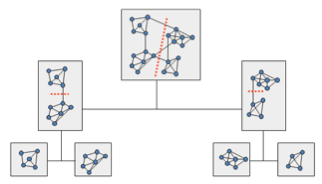
\includegraphics[width=0.5\textwidth]{recursive_split.png}
    \label{fig:recursive_split}
    \caption{The recursion tree for the successive splitting of some graph.}
\end{figure}

Other optimality criteria can be applied in graph clustering: \begin{description}
    \item[modularity]
    $$ \text{modularity} =
        \frac{1}{2m} \sum_{u,v\in V} 1_{c_u=c_v}
            (A_{uv} - (2m)^{-1} \delta_v \delta_u)\,,$$
    where $c_v$ is the cluster of the node $v$; in a two-cluster case $1_{c_u=c_v}
    = \frac{1}{2}(s_u s_v + 1)$, whence
    $$ \text{modularity} = \frac{1}{4m} s'(A - A \one (2m)^{-1} \one'A) s\,,$$
    with $s\in \{-1,1\}^V$, $s's = |V|$ and $m$ -- the number of edges.
\end{description}
Since the modularity metric is maximized, we seek the eigenvector with the largest eigenvalue.

\hfill\\\textbf{Q:}\rus{Предмет и задачи машинного обучения и разработки (майнинга)
данных. Таксономия методов. Примеры задач.}

\hfill\\\textbf{A:}

% section mldm (end)

\end{document}
